%==========================================================================
% PHY 104 -- Periodic Motion
% Combined Lecture Slide Deck
% Author: Albert Ndulue
%==========================================================================
\documentclass[aspectratio=169,xcolor=dvipsnames]{beamer}

\usepackage{beamertheme_um}
\usepackage[utf8]{inputenc}
\usepackage[T1]{fontenc}
\usepackage{amsmath}
\usepackage{siunitx}
\usepackage{booktabs}
\usepackage{array}
\usepackage{multicol}
\usepackage{pgfplots}
\pgfplotsset{compat=1.18}
\usetikzlibrary{decorations.pathmorphing,patterns,angles,quotes,arrows.meta}
\usepackage{cleveref}

%--------------------------------------------------------------------------
% Metadata
%--------------------------------------------------------------------------
\title[Periodic Motion]{Periodic Motion}
\subtitle{Concepts, derivations, and why oscillations matter}
\author[Albert Ndulue]{Albert Ndulue}
\institute[PHY 104]{Department of Physics}
\date{\today}

%--------------------------------------------------------------------------
% Section divider slide definition
%--------------------------------------------------------------------------
\AtBeginSection{%
  \begin{frame}[plain]
    \begin{tikzpicture}[remember picture,overlay]
      \fill[top color=slidebg,bottom color=ocredark]
        (current page.south west) rectangle (current page.north east);
      \node[anchor=south west,opacity=0.09]
        at ([xshift=4mm]current page.south west)
        {\color{white}\fontsize{190}{190}\selectfont\sffamily\bfseries
         \thesection};
      \draw[ocre,line width=0.8pt]
        ([xshift=8mm,yshift=-0.37\paperheight]current page.west) --
        ([xshift=-8mm,yshift=-0.37\paperheight]current page.east);
      \node[anchor=south west,font=\small\sffamily\bfseries,text=ocrelight]
        at ([xshift=8mm,yshift=-0.37\paperheight+3mm]current page.west)
        {\MakeUppercase{Section \thesection}};
      \node[anchor=north west,text width=0.84\paperwidth,align=left,
            font=\Large\sffamily\bfseries,text=white]
        at ([xshift=8mm,yshift=-0.37\paperheight-4mm]current page.west)
        {\insertsectionhead};
    \end{tikzpicture}
  \end{frame}
}

%==========================================================================
\begin{document}
%==========================================================================

\begin{frame}[plain]
  \titlepage
\end{frame}

\begin{frame}{Pre-Class Quiz}
  \begin{columns}[c]
    \begin{column}{0.58\textwidth}
      Before we begin, please scan the QR code to complete the pre-class quiz:
      \vspace{0.8em}
      \begin{itemize}
        \item Pinpoint your prior understanding of periodic motion.
        \item Highlight common misconceptions for class discussion.
        \item Responses will be projected at the start of class.
      \end{itemize}
    \end{column}
    \hfill
    \begin{column}{0.36\textwidth}
      \centering
      
\includegraphics[width=\textwidth,keepaspectratio]{pre-class quiz.png}
    \end{column}
  \end{columns}
\end{frame}

%--------------------------------------------------------------------------
% Outline Slide matching Obsidian note structure
%--------------------------------------------------------------------------
\begin{frame}{Outline}
  \begin{columns}[T]
    \begin{column}{0.54\textwidth}
      \large
      \begin{itemize}
        \item[\color{lawcolor}\checkmark] Introduction
        \item[\color{lawcolor}\checkmark] What is Oscillation
        \item[\color{lawcolor}\checkmark] Harmonic Oscillation
        \item[\color{lawcolor}\checkmark] Terminologies in SHM
        \item[\color{lawcolor}\checkmark] Energy in SHM
        \item[\color{lawcolor}\checkmark] Linearity and Time-Translation Invariance
        \item[\color{lawcolor}\checkmark] The Complex Exponential and Rotating Phasors
        \item[\color{lawcolor}\checkmark] Solving the equation of motion of SHM
        \item[\color{lawcolor}\checkmark] Other Common Oscillators
      \end{itemize}
    \end{column}
    \begin{column}{0.40\textwidth}
      \begin{umnote}[Learning Arc]
        We align the lecture with our study guide. We focus on conceptual definitions first, and then build the mathematical framework step-by-step.
      \end{umnote}
    \end{column}
  \end{columns}
\end{frame}

%==========================================================================
\section{Introduction}
%==========================================================================

\begin{frame}{A Moment of Pondering}
  \begin{columns}[c]
    \begin{column}{0.58\textwidth}
      \begin{umlaw}{Nikola Tesla}
        \small ``If you want to find the secrets of the universe, think in terms of energy, frequency, and vibration.''
      \end{umlaw}
      \vspace{0.2em}
      \begin{itemize}
        \item Before we begin, close your eyes, cover your ears, sit in silence for a minute, and ponder this saying.
        \item What did you observe? A silent void, perhaps.
        \item But even that silence tells us something important.
      \end{itemize}
    \end{column}
    \hfill
    \begin{column}{0.36\textwidth}
      \centering
      \vfill
      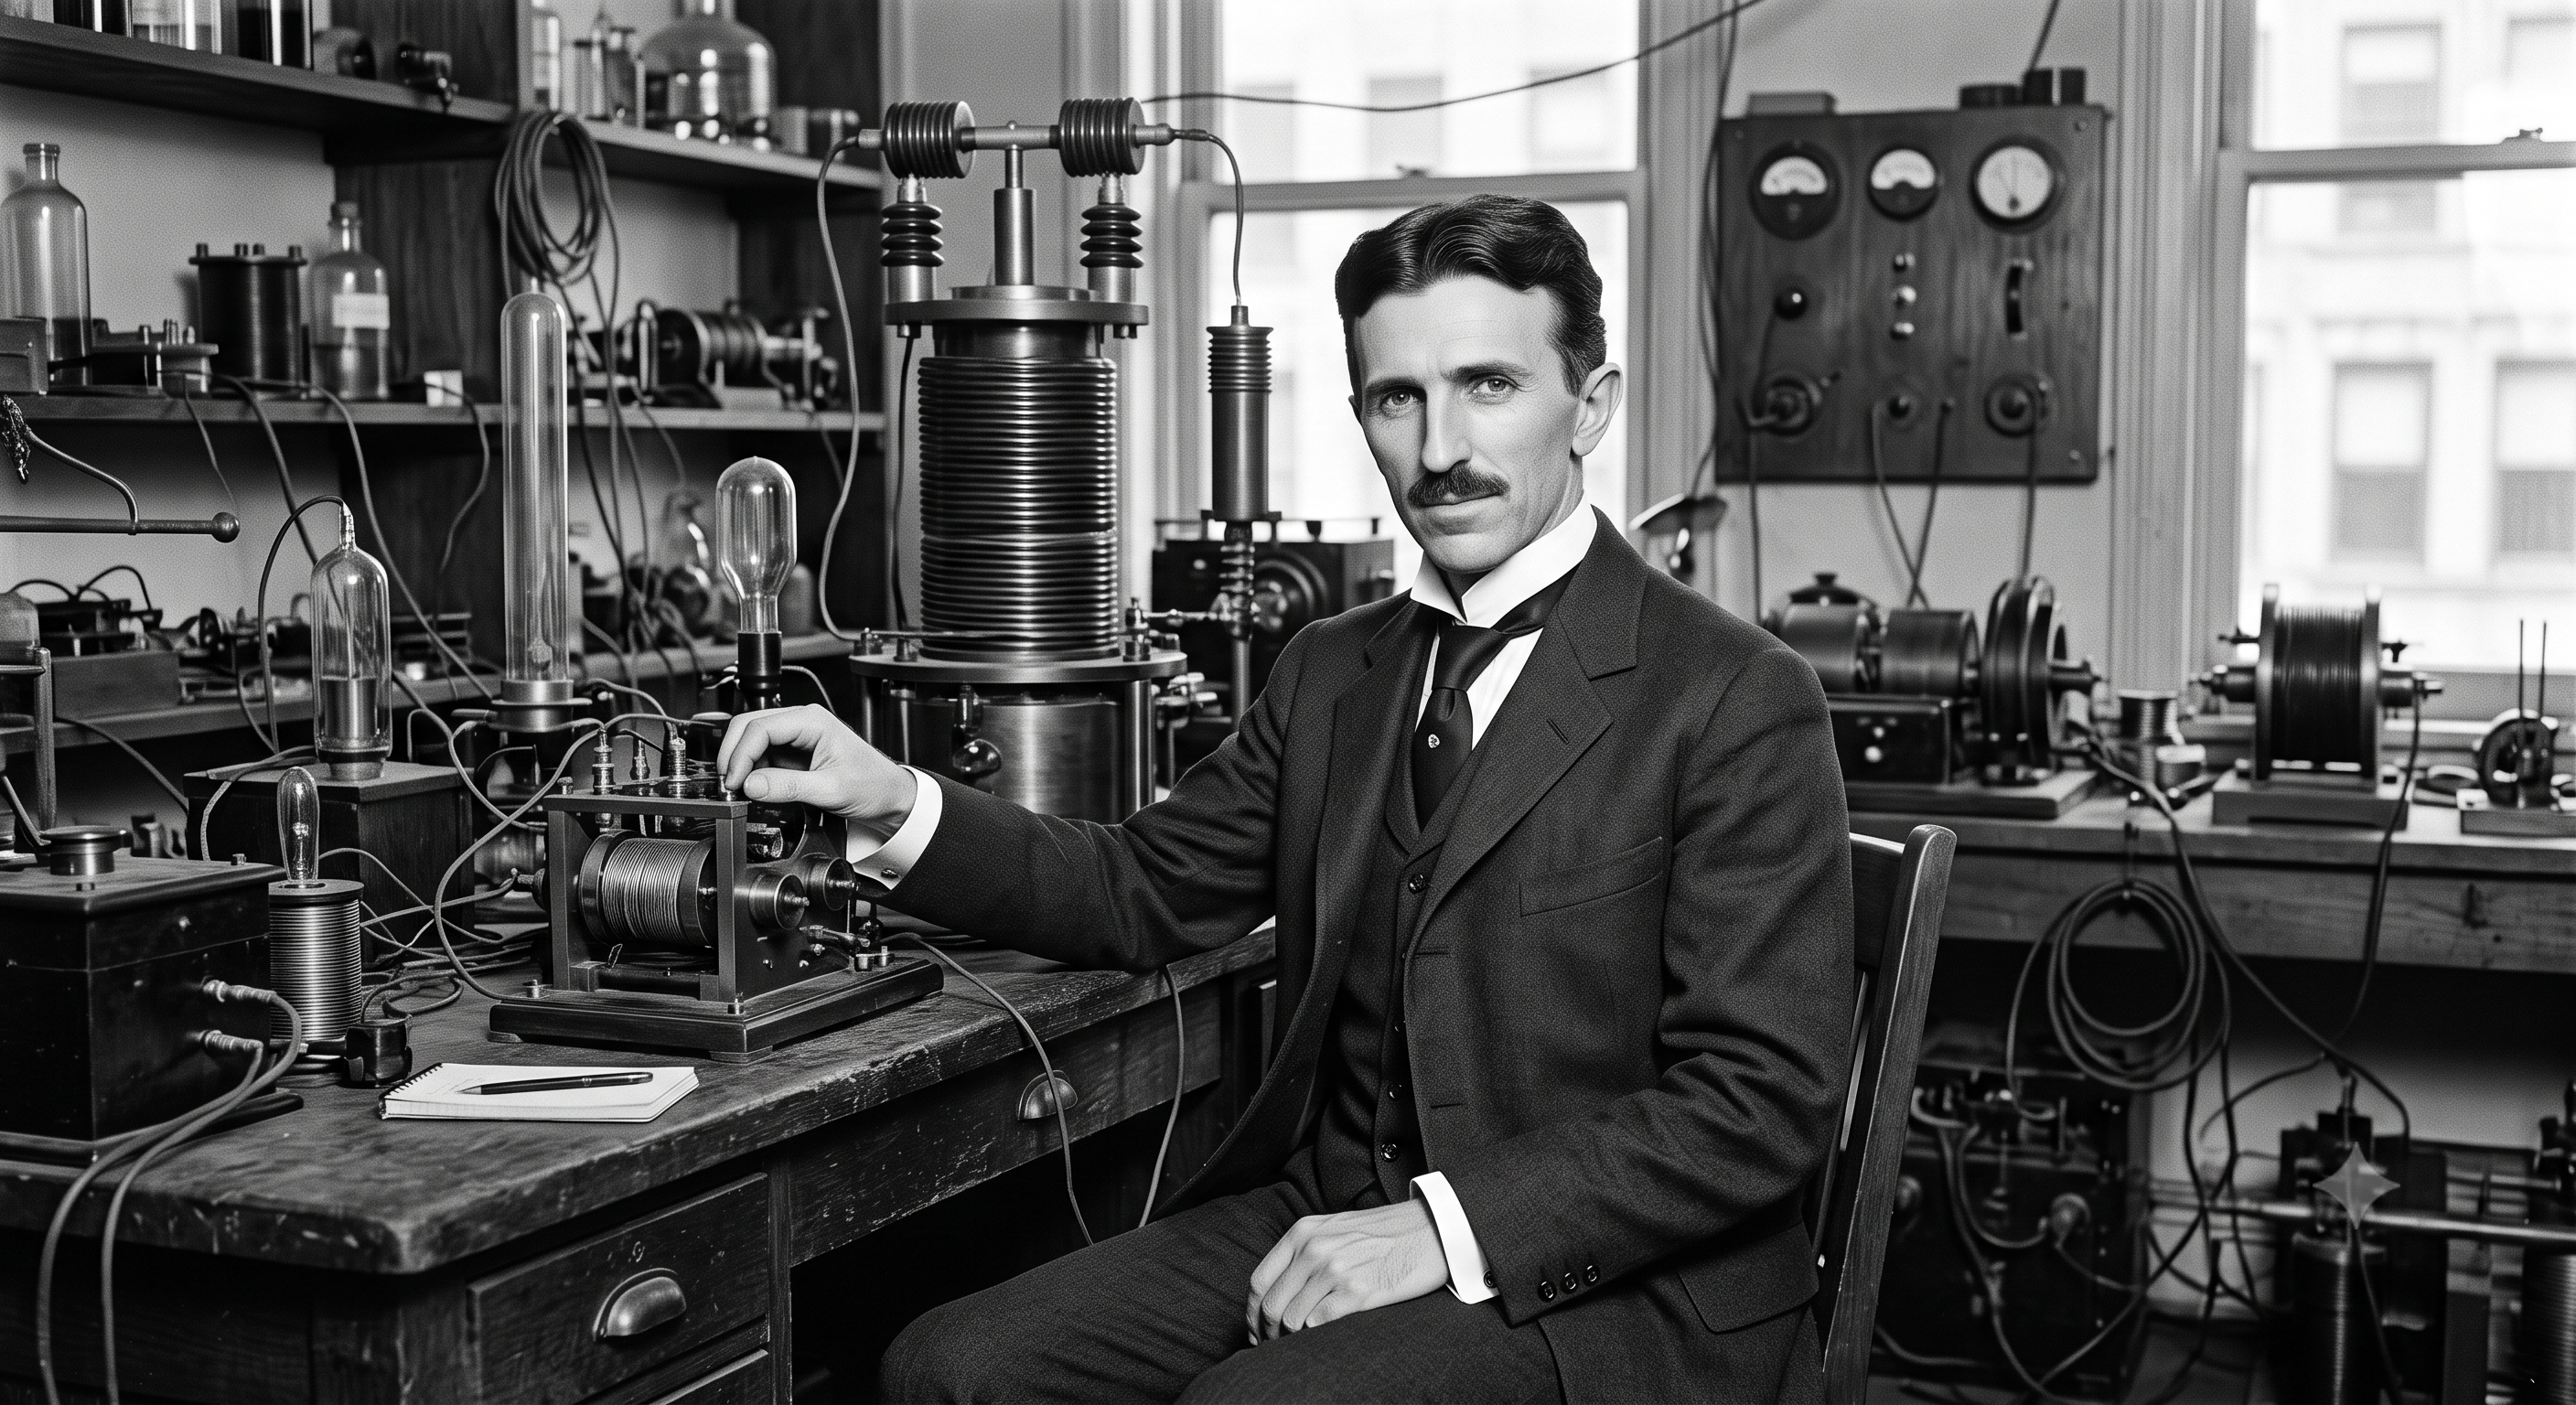
\includegraphics[width=\textwidth,keepaspectratio]{nikola_tesla.png}
      \vfill
    \end{column}
  \end{columns}
\end{frame}

\begin{frame}{Silence vs. Oscillation}
  \begin{columns}[c]
    \begin{column}{0.58\textwidth}
      \begin{itemize}
        \item \textbf{Sound} depends on the oscillation and vibration of particles in a medium.
        \item \textbf{Light} depends on oscillating electric and magnetic fields.
        \item The universe would be a silent, uninteresting void without oscillations.
      \end{itemize}

      \vspace{0.8em}
      \begin{umnote}[Fundamental Question]
        What makes oscillations so special? Why do so many physical phenomena depend on oscillation and wave motion?
      \end{umnote}
    \end{column}
    \hfill
    \begin{column}{0.36\textwidth}
      \centering
      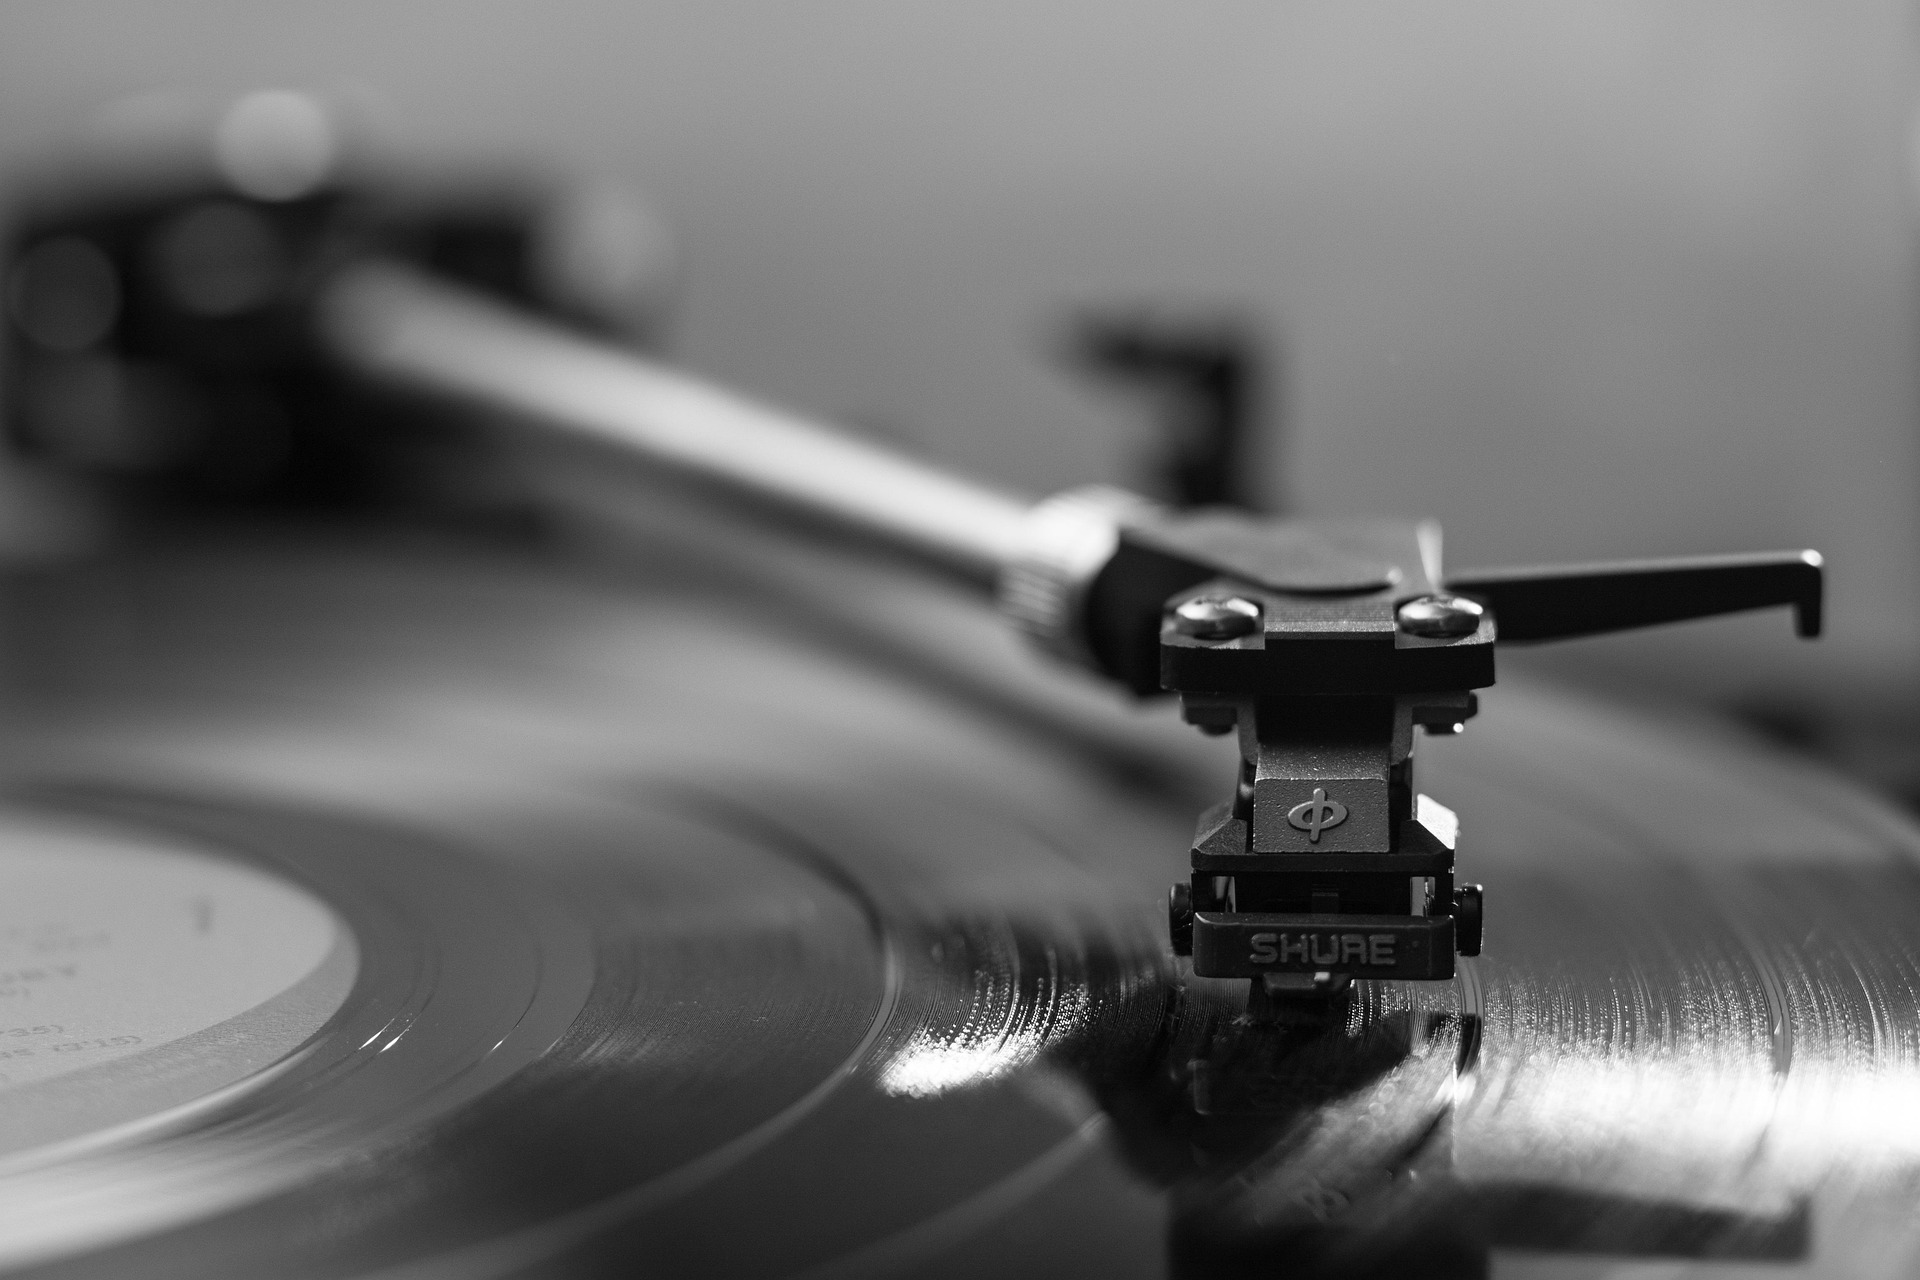
\includegraphics[width=\textwidth,keepaspectratio]{pexels-record-player.jpg}
      \vskip 0.2em
      \tiny Photo credit: Pexels
    \end{column}
  \end{columns}
\end{frame}

\begin{frame}{Why It Matters for Engineering}
  \begin{columns}[T]
    \begin{column}{0.48\textwidth}
      \begin{umlaw}{Useful Applications}
        Oscillations make many technologies possible:
        \begin{itemize}
          \item Sound systems and acoustics
          \item Sensors and instrumentation
          \item Rotating and vibrating machinery
          \item Telecommunications
        \end{itemize}
      \end{umlaw}
    \end{column}
    \begin{column}{0.48\textwidth}
      \begin{umlaw}{Engineering Hazards}
        If left unchecked, vibrations can:
        \begin{itemize}
          \item Damage machinery
          \item Fatigue and weaken materials
          \item Cause structural failure (e.g., bridge collapses)
        \end{itemize}
      \end{umlaw}
    \end{column}
  \end{columns}
\end{frame}

\begin{frame}{Our Quest in This Course}
  We begin our quest to obtain answers to these key questions:
  \begin{enumerate}
    \item What are the fundamental building blocks of vibrations?
    \item What are the energy consequences of vibrations?
    \item What happens when vibrations propagate from one place to another?
    \item How can we employ, as well as control, vibrations to improve our lives?
  \end{enumerate}

  \vspace{0.8em}
  \begin{umnote}[The Language of Nature]
    By the end of this course, you should not see vibrations and waves as just formulas on a board. You should see them as one of the basic languages through which nature, machines, and engineering systems communicate.
  \end{umnote}
\end{frame}

%==========================================================================
\section{What is Oscillation?}
%==========================================================================

\begin{frame}{Periodic Motion vs. Oscillation}
  \begin{umdefinition}{Periodic Motion}
    Any motion that repeats itself after a specific time interval is called a \textbf{periodic motion}. Its position at a given time repeats itself after a fixed time interval, called the \textbf{period} $T$.
  \end{umdefinition}

  \begin{umformula}
    \begin{equation}
      x(t) = x(t + T)
    \end{equation}
  \end{umformula}

  \begin{umdefinition}{Oscillation}
    An \textbf{oscillation} is a subset of periodic motion. It is the repeated variation of a physical quantity about an equilibrium or mean value.
  \end{umdefinition}
\end{frame}

\begin{frame}{Equilibrium and Restoring Force}
  \begin{columns}[c]
    \begin{column}{0.5\textwidth}
      \begin{itemize}
        \item In a mechanical system, oscillation appears as the to-and-fro motion of a particle about its equilibrium position.
        \item \textbf{Equilibrium Position:} The position where the net force on the particle is zero.
        \item \textbf{Restoring Force:} A force that tends to bring the particle back toward equilibrium whenever it is displaced.
        \item If an oscillation occurs in a mechanical system, it is usually called a \textbf{vibration}.
      \end{itemize}
    \end{column}
    \begin{column}{0.4\textwidth}
      \centering
      \vfill
      \begin{tikzpicture}[scale=0.75]
        \draw[thick] (-0.2,0.8) -- (-0.2,-0.8);
        \foreach \y in {-0.75,-0.5,...,0.75}
        \draw (-0.28,\y) -- (-0.5,\y-0.12);
        \draw[decorate,decoration={coil,aspect=0.45,segment length=5pt,amplitude=4pt},
          thick,ocre] (-0.2,0) -- (2.2,0);
        \draw[thick,fill=ocrelight] (2.2,-0.45) rectangle (3.1,0.45);
        \draw[->,thick,dexpiRedDark] (2.65,0) -- (3.65,0)
        node[right] {\small displacement \(x\)};
        \draw[->,thick,lawcolor] (2.65,-0.15) -- (1.55,-0.15)
        node[below] {\small restoring force};
      \end{tikzpicture}
      \vfill
      \begin{umnote}[Horizontal Mass-Spring]
        A mass on a frictionless surface is a classic mechanical oscillator.
      \end{umnote}
      \vfill
    \end{column}
  \end{columns}
\end{frame}

\begin{frame}{The Mechanics of Overshooting}
  How does the oscillation sustain itself?
  \begin{enumerate}
    \item \textbf{Displacement:} Displace the mass from equilibrium. The spring stretches and exerts a restoring force towards equilibrium.
    \item \textbf{Acceleration:} Released from rest, the mass accelerates toward the equilibrium position.
    \item \textbf{Overshoot:} At equilibrium, the net force is zero, but the mass has gained velocity and inertia. It overshoots the equilibrium position.
    \item \textbf{Compression:} The spring compresses, exerting a restoring force in the opposite direction, slowing the mass down until it stops and reverses.
    \item \textbf{Ideal Oscillation:} Without friction or energy loss, this cycle continues indefinitely.
  \end{enumerate}
\end{frame}

%==========================================================================
\section{Harmonic Oscillation}
%==========================================================================

\begin{frame}{Hooke's Law}
  \begin{umdefinition}{Harmonic Oscillation}
    For an oscillation to be harmonic, the restoring force must be directly proportional to the displacement from equilibrium:
    \begin{equation}
      F = -k(x - x_0)
    \end{equation}
    where $k$ is the \textbf{force constant} and $x_0$ is the equilibrium position.
  \end{umdefinition}
\end{frame}

\begin{frame}{Hooke's Law}
  \begin{itemize}
    \item This is a statement of \textbf{Hooke's Law}. A system obeying this is a \textbf{harmonic oscillator}.
    \item The minus sign indicates the restoring force acts in the opposite direction of displacement.
    \item \textbf{Idealization:} Hooke's law is an approximation, but works exceptionally well for sufficiently small displacements.
  \end{itemize}
\end{frame}


\begin{frame}{Derivation: Equation of Motion}
  Let us derive the differential equation for a simple harmonic oscillator. Set the coordinate origin at the equilibrium position ($x_0 = 0$):
  \vspace{0.5em}

  \begin{align*}
    \onslide<1->{F           & = -kx \tag{Hooke's Law} \\}
    \onslide<2->{F           & = ma} \only<2->{\tag{Newton's Second Law}}        \\
    \onslide<3->{\implies ma & = -kx}
  \end{align*}
\end{frame}

\begin{frame}{Derivation: Equation of Motion}
  Since $a = \frac{d^2}{dt^2}x(t)$, we have:
  \begin{equation*}
    m \frac{d^2}{dt^2}x(t) = -kx(t)
  \end{equation*}

  \pause
  \vspace{0.8em}
  Rearranging terms gives:
  \begin{equation}
    \boxed{m \frac{d^2}{dt^2}x(t) + kx(t) = 0}
    \label{eq:sho-eom}
  \end{equation}
\end{frame}

\begin{frame}{What is a ``Simple'' Harmonic Oscillator?}
  The equation we derived:
  \[
    m \frac{d^2x(t)}{dt^2} + kx(t) = 0
  \]
  \vspace{0.8em}
  \begin{umnote}[Simple Harmonic Oscillator (SHO)]
    The word \textbf{``Simple''} implies that the system is:
    \begin{itemize}
      \item \textbf{Free:} No external forces acting on it.
      \item \textbf{Undamped:} No friction, air resistance, or mechanical energy loss.
      \item \textbf{Unforced:} No driving forces pushing the system.
      \item \textbf{Linear:} The restoring force is directly proportional to displacement.
    \end{itemize}
  \end{umnote}
\end{frame}

\begin{frame}{General Solution}
  \cref{eq:sho-eom} is a second-order, linear differential equation. The proposed general solution is:
  \vspace{0.5em}
  \begin{umformula}{Proposed General Solution}
    \begin{equation}
      x(t) = c_1 \cos(\omega t) + c_2 \sin(\omega t)
      \label{eq:general-solution}
    \end{equation}
  \end{umformula}
  \begin{itemize}
    \item $c_1$ and $c_2$ are arbitrary constants determined by the initial displacement and velocity of the particle.
    \item $\omega$ is the \textbf{angular frequency} of the oscillation, given by:
          \[
            \omega = \sqrt{\frac{k}{m}}
          \]
  \end{itemize}
\end{frame}

\begin{frame}{Derivation: Verifying the Solution (Part 1)}
  To prove that our proposed $x(t) = c_1 \cos(\omega t) + c_2 \sin(\omega t)$ is a solution, we first compute its derivatives:
  \vspace{0.5em}
  \begin{align*}
    \onslide<1->{x'(t)  & = \frac{d}{dt}\left[ c_1 \cos(\omega t) + c_2 \sin(\omega t) \right] \\}
    \onslide<2->{       & = \omega \left[ -c_1 \sin(\omega t) + c_2 \cos(\omega t) \right] \\}
    \onslide<3->{x''(t) & = \frac{d}{dt}\left[ x'(t) \right] \\}
    \onslide<4->{       & = -\omega^2 \left[ c_1 \cos(\omega t) + c_2 \sin(\omega t) \right] \\}
    \onslide<5->{       & = -\omega^2 x(t)}
  \end{align*}
\end{frame}

\begin{frame}{Derivation: Verifying the Solution (Part 2)}
  Now, substitute $x''(t) = -\omega^2 x(t)$ back into the equation of motion:
  \[
    m \frac{d^2x(t)}{dt^2} + kx(t) = 0
  \]
  \pause
  \begin{align*}
    \onslide<2->{m(-\omega^2 x(t)) + k x(t)   & = 0 \\}
    \onslide<3->{\implies (k - m\omega^2)x(t) & = 0}
  \end{align*}
  \onslide<4->
  This equation must hold for all times $t$. This is true if and only if the coefficient is zero:
  \begin{umformula}
    \[
      k - m\omega^2 = 0 \implies \omega^2 = \frac{k}{m} \implies \omega = \sqrt{\frac{k}{m}}
    \]
  \end{umformula}
\end{frame}

\begin{frame}{Derivation: Releasing from Rest}
  For the unique case where the particle is released from rest at maximum displacement $A$:
  \[
    \text{Initial Conditions:} \quad x(0) = A, \quad x'(0) = 0
  \]
  \pause
  Substitute into the general solution at $t = 0$:
  \begin{align*}
    \onslide<2->{x(0) & = c_1 \cos(0) + c_2 \sin(0) \\}
    \onslide<3->{     & = c_1 + 0 = A \implies c_1 = A}
  \end{align*}
  \onslide<4->
  Substitute into the velocity expression $x'(t)$ at $t = 0$:
  \begin{align*}
    \onslide<4->{x'(0) & = \omega \left[ -c_1 \sin(0) + c_2 \cos(0) \right] \\}
    \onslide<5->{      & = \omega c_2 = 0 \implies c_2 = 0 \quad (\text{since } \omega \neq 0)}
  \end{align*}
  \onslide<6->
  This yields the particular solution: \quad \boxed{x(t) = A \cos(\omega t)}
\end{frame}

%==========================================================================
\section{Key Terminologies}
%==========================================================================

\begin{frame}{Key Terminologies: Amplitude, Period, \& Frequency}
  \begin{columns}[T]
    \begin{column}{0.48\textwidth}
      \begin{umdefinition}{Amplitude \& Period}
        \begin{itemize}
          \item \textbf{Amplitude ($A$):} The maximum displacement from equilibrium.
          \item \textbf{Period ($T$):} The time taken to complete one full cycle (measured in seconds, $\text{s}$).
        \end{itemize}
      \end{umdefinition}
      \begin{umnote}[Physical Example]
        \small In a mass-spring system, $T$ is the time to complete one full cycle of motion.
      \end{umnote}
    \end{column}
    \begin{column}{0.48\textwidth}
      \begin{umdefinition}{Frequency}
        The number of complete cycles per unit time, measured in hertz ($\text{Hz}$).

        \vspace{0.5em}
        \textbf{Relationship:}
        \[
          f = \frac{1}{T}
        \]
      \end{umdefinition}
    \end{column}
  \end{columns}
\end{frame}

\begin{frame}{Key Terminologies: Angular Frequency \& Phase}
  \begin{columns}[T]
    \begin{column}{0.48\textwidth}
      \begin{umdefinition}{Angular Frequency}
        The rate of change of the phase angle, measured in radians per second ($\text{rad/s}$).

        \vspace{0.5em}
        \textbf{Relationship to $f$:}
        \[
          \omega = 2\pi f = \frac{2\pi}{T}
        \]
      \end{umdefinition}
    \end{column}
    \begin{column}{0.48\textwidth}
      \begin{umdefinition}{Phase \& Phase Constant}
        \begin{itemize}
          \item \textbf{Phase ($\Phi(t)$):} The angular argument indicating where the oscillator is in its cycle at time $t$.
          \item \textbf{Phase Constant ($\phi$):} The initial phase at $t=0$.
        \end{itemize}

        \vspace{0.5em}
        \textbf{Phase Equation:}
        \[
          \Phi(t) = \omega t + \phi \implies \Phi(0) = \phi
        \]
      \end{umdefinition}
    \end{column}
  \end{columns}
\end{frame}

%==========================================================================
\section{Energy in a Simple Harmonic Oscillator}
%==========================================================================

\begin{frame}{Energy Exchange in SHM}
  \begin{columns}[T]
    \begin{column}{0.5\textwidth}
      \begin{itemize}
        \item As a system oscillates, mechanical energy continuously flows between \textbf{Potential Energy} ($U$) and \textbf{Kinetic Energy} ($K$).
        \item In a simple harmonic oscillator, we neglect:
              \begin{itemize}
                \item Damping and friction
                \item Air resistance
                \item External driving forces
              \end{itemize}
        \item The restoring force is conservative, so the total mechanical energy $E$ remains \textbf{constant}.
      \end{itemize}
    \end{column}
    \begin{column}{0.46\textwidth}
      \begin{umnote}[The Cycle of Energy]
        \small
        \begin{itemize}
          \item \textbf{At amplitudes ($x = \pm A$):} Velocity is zero $\implies K = 0$. Potential energy is maximum.
          \item \textbf{At equilibrium ($x = 0$):} Restoring force is zero, speed is maximum $\implies K$ is maximum. Potential energy is minimum ($U = 0$).
          \item \textbf{In between:} Energy is shared: $E = K + U$.
        \end{itemize}
      \end{umnote}
    \end{column}
  \end{columns}
\end{frame}

\begin{frame}{Derivation: Potential Energy $U(x)$}
  A conservative restoring force $F(x)$ relates to the potential energy function $U(x)$ by:
  \begin{equation*}
    F(x) = -\frac{dU}{dx} \implies U(x) = -\int F(x) \, dx + C
  \end{equation*}
  \pause
  For our Hooke's Law force, $F(x) = -kx$:
  \begin{equation*}
    U(x) = \int kx \, dx + C = \frac{1}{2}kx^2 + C
  \end{equation*}
  \pause
  Setting $U(0) = 0$ as our reference ($C = 0$):
  \begin{umformula}
    \textbf{Potential Energy:} \quad $\boxed{U(x) = \frac{1}{2}kx^2}$
  \end{umformula}
\end{frame}

\begin{frame}{Derivation: Total Energy and Speed}
  The total mechanical energy $E$ is constant, and is the sum of potential and kinetic energy ($K = \frac{1}{2}mv^2$):
  \begin{equation*}
    E = U + K = \frac{1}{2}kx^2 + \frac{1}{2}mv^2
  \end{equation*}
  \pause
  At maximum displacement ($x = A$), speed $v = 0$: \quad $E = \frac{1}{2}kA^2$
  \pause
  Equating these gives:
  \begin{equation*}
    \frac{1}{2}mv^2 = \frac{1}{2}k(A^2 - x^2) \implies v^2 = \frac{k}{m}(A^2 - x^2)
  \end{equation*}
  \begin{umformula}
    \textbf{Speed vs. Position:} \quad $\boxed{|v| = \omega\sqrt{A^2 - x^2}}$ \quad where $\omega = \sqrt{\frac{k}{m}}$
  \end{umformula}
\end{frame}

\begin{frame}{Energy as a Function of Time}
  Substitute the solution $x(t) = A\cos(\omega t)$ and velocity $v(t) = -A\omega\sin(\omega t)$ into our energy equations:
  \vspace{-0.5em}
  \begin{align*}
    U(t) & = \frac{1}{2}kA^2\cos^2(\omega t)                                            \\
    K(t) & = \frac{1}{2}m\omega^2 A^2\sin^2(\omega t)                                   \\
    E(t) & = \frac{1}{2}kA^2\cos^2(\omega t) + \frac{1}{2}m\omega^2 A^2\sin^2(\omega t)
  \end{align*}
  Since $m\omega^2 = k$, the total energy remains constant: $E(t) = \frac{1}{2}kA^2$.
\end{frame}

\begin{frame}{Graphical Representation of Energy}
  \begin{columns}[T]
    \begin{column}{0.48\textwidth}
      \begin{itemize}
        \item \textbf{Potential Energy $U(t)$:} Oscillates as $\cos^2(\omega t)$ (solid blue line).
        \item \textbf{Kinetic Energy $K(t)$:} Oscillates as $\sin^2(\omega t)$ (solid green line).
        \item \textbf{Total Energy $E$:} Constant at $\frac{1}{2}kA^2$ (dashed black line).
        \item \textbf{Key Observation:} $U(t)$ and $K(t)$ are exactly $90^\circ$ out of phase. The frequency of energy oscillation is $2\omega$ (double the motion frequency).
      \end{itemize}
    \end{column}
    \begin{column}{0.48\textwidth}
      \centering
      \begin{tikzpicture}[scale=0.85]
        \begin{axis}[
            axis lines = left,
            xlabel = {Time $\omega t$},
            ylabel = {Energy},
            xmin=0, xmax=360,
            ymin=0, ymax=1.2,
            xtick={0, 90, 180, 270, 360},
            xticklabels={$0$, $\frac{\pi}{2}$, $\pi$, $\frac{3\pi}{2}$, $2\pi$},
            ytick={0, 1},
            yticklabels={$0$, $\frac{1}{2}kA^2$},
            legend style={at={(0.5, 1.15)}, anchor=south, legend columns=-1, draw=none, fill=none},
            width=7.2cm,
            height=4.8cm,
            every axis x label/.style={at={(current axis.right of origin)},anchor=north west},
            every axis y label/.style={at={(current axis.above origin)},anchor=south east}
          ]
          \addplot [
            domain=0:360,
            samples=100,
            color=ocre,
            thick
          ] {(cos(x))^2};
          \addlegendentry{$U(t)$}

          \addplot [
            domain=0:360,
            samples=100,
            color=lawcolor,
            thick
          ] {(sin(x))^2};
          \addlegendentry{$K(t)$}

          \addplot [
            domain=0:360,
            samples=10,
            color=black,
            dashed,
            thick
          ] {1};
          \addlegendentry{$E$}
        \end{axis}
      \end{tikzpicture}
    \end{column}
  \end{columns}
\end{frame}

\begin{frame}{Derivation: Consistency of Energy Conservation}
  For total energy $E(t)$ to remain constant ($\frac{1}{2}kA^2$) for all time $t$:
  \[
    \frac{1}{2}kA^2\cos^2(\omega t) + \frac{1}{2}m\omega^2 A^2\sin^2(\omega t) = \frac{1}{2}kA^2
  \]
  \pause
  Factor out $\frac{1}{2}A^2$ and use $\sin^2(\omega t) = 1 - \cos^2(\omega t)$:
  \begin{align*}
    k\cos^2(\omega t) + m\omega^2\left[1 - \cos^2(\omega t)\right] & = k             \\
    \implies (k - m\omega^2)\cos^2(\omega t) + m\omega^2           & = k             \\
    \implies (k - m\omega^2)\cos^2(\omega t)                       & = k - m\omega^2
  \end{align*}
  \pause
  For this to hold true for all $t \in \mathbb{R}$, we must have:
  \[
    k - m\omega^2 = 0 \implies \omega^2 = \frac{k}{m} \implies \omega = \sqrt{\frac{k}{m}}
  \]
  This confirms that energy conservation is consistent with our solution!
\end{frame}

%==========================================================================
\section{Linearity and Time-Translation Invariance}
%==========================================================================

\begin{frame}{Mathematical Foundations}
  \begin{columns}[c]
    \begin{column}{0.58\textwidth}
      Before deriving the general solution of the simple harmonic oscillator, we examine two powerful features of its equation of motion:
      \vspace{0.5em}
      \[
        m\frac{d^2x}{dt^2} + kx = 0
      \]
      \vspace{0.5em}
      \begin{itemize}
        \item \textbf{Linearity}
        \item \textbf{Time-Translation Invariance}
      \end{itemize}
    \end{column}
    \hfill
    \begin{column}{0.36\textwidth}
      \begin{umnote}[Why this matters]
        These two symmetries simplify the mathematics and explain why harmonic oscillators appear universally in physics and engineering.
      \end{umnote}
    \end{column}
  \end{columns}
\end{frame}

\begin{frame}{Linearity \& Superposition}
  \begin{umdefinition}{Linearity}
    A differential equation is \textbf{linear} if the dependent variable $x(t)$ and its derivatives appear only to the first power, with no products or nonlinear functions (e.g., $x^2$, $\sin x$, $x \dot{x}$).
  \end{umdefinition}
  \pause
  \vspace{0.4em}
  \begin{umnote}[Principle of Superposition]
    If $x_1(t)$ and $x_2(t)$ are both solutions to a linear differential equation, then any linear combination $x(t) = a x_1(t) + b x_2(t)$ is also a solution (where $a$ and $b$ are constants).
  \end{umnote}
  \pause
  \vspace{0.4em}
  Since $\cos(\omega t)$ and $\sin(\omega t)$ are solutions, their combination $c_1\cos(\omega t) + c_2\sin(\omega t)$ is also a solution.
\end{frame}

\begin{frame}{Time-Translation Invariance}
  \begin{columns}[T]
    \begin{column}{0.5\textwidth}
      \begin{umlaw}{Time-Translation Invariance}
        The physics of the system does not depend on the specific starting time of observation. The equation of motion contains no explicit time dependence:
        \[
          m\frac{d^2x}{dt^2} + kx = 0
        \]
        This is an \textbf{autonomous equation}.
      \end{umlaw}
    \end{column}
    \hfill
    \begin{column}{0.46\textwidth}
      \begin{itemize}
        \item If $x(t)$ is a solution, then $x(t+\alpha)$ is also a solution for any time shift $\alpha$.
        \item Shift of time origin is equivalent to a phase shift:
              \[
                \begin{aligned}
                  x(t+\alpha) &= A\cos(\omega(t+\alpha)) \\
                              &= A\cos(\omega t + \phi)
                \end{aligned}
              \]
              where $\phi = \omega\alpha$ is the phase constant.
      \end{itemize}
    \end{column}
  \end{columns}
\end{frame}

%==========================================================================
\section{The Complex Exponential and Rotating Phasors}
%==========================================================================

\begin{frame}{The Search for Irreducible Solutions}
  \begin{columns}[T]
    \begin{column}{0.60\textwidth}
      Shifting $t \to t+\alpha$ in sines/cosines mixes terms:
      \begin{align*}
        x(t+\alpha) &= c_1 \cos\omega(t+\alpha) + c_2 \sin\omega(t+\alpha) \\
        &= c_1 [\cos\omega t\cos\omega\alpha - \sin\omega t\sin\omega\alpha] \\
        &\quad + c_2 [\sin\omega t\cos\omega\alpha + \cos\omega t\sin\omega\alpha] \\
        &= [c_1\cos\phi + c_2\sin\phi]\cos\omega t \\
        &\quad + [c_2\cos\phi - c_1\sin\phi]\sin\omega t \\
        &= c_3 \cos\omega t + c_4 \sin\omega t
      \end{align*}
      where $\phi = \omega\alpha$, $c_3 = c_1\cos\phi + c_2\sin\phi$, and $c_4 = c_2\cos\phi - c_1\sin\phi$.
    \end{column}
    \hfill
    \begin{column}{0.36\textwidth}
      \begin{umnote}[Why it is messy]
        Proving time-translation invariance with sines/cosines is algebraically tedious.
      \end{umnote}
      \begin{itemize}
        \item We seek an \textbf{irreducible solution} satisfying $x(t+\alpha) = h(\alpha)x(t)$.
        \item The solution is the \textbf{complex exponential}.
      \end{itemize}
    \end{column}
  \end{columns}
\end{frame}

\begin{frame}{Complex Numbers Review}
  \begin{columns}[T]
    \begin{column}{0.48\textwidth}
      \begin{umdefinition}{Complex Number}
        A complex number $z$ consists of a real part $a$ and an imaginary part $b$:
        \[
          z = a + ib \quad \text{where} \quad i = \sqrt{-1}
        \]
      \end{umdefinition}
      \begin{itemize}
        \item \textbf{Conjugate:} $z^* = a - ib$
        \item \textbf{Modulus (Magnitude):} $r = \sqrt{a^2 + b^2}$
        \item \textbf{Argument (Angle):} $\theta = \tan^{-1}(b/a)$
      \end{itemize}
    \end{column}
    \hfill
    \begin{column}{0.48\textwidth}
      \centering
      \begin{tikzpicture}[scale=0.9, >=Stealth]
        \draw[->,thick] (-0.5,0) -- (3.2,0) node[right] {\small Re};
        \draw[->,thick] (0,-0.5) -- (0,2.6) node[above] {\small Im};
        \coordinate (Z) at (2.4,1.8);
        \draw[->,ultra thick,ocre] (0,0) -- (Z) node[above right] {$z = a + ib$};
        \draw[dashed,gray] (2.4,0) -- (Z);
        \draw[dashed,gray] (0,1.8) -- (Z);
        \draw (0.6,0) arc (0:36.87:0.6) node[midway,right,yshift=1.5pt] {$\theta$};
        \node[below] at (1.2,0) {$a$};
        \node[left] at (0,0.9) {$b$};
        \node[above left,ocre] at (1.2,0.9) {$r$};
      \end{tikzpicture}
      \begin{umformula}
        \centering Polar Form: \quad $z = r(\cos\theta + i\sin\theta)$
      \end{umformula}
    \end{column}
  \end{columns}
\end{frame}

\begin{frame}{Euler's Formula}
  Let us examine the derivative of $\cos\theta + i\sin\theta$:
  \[
    \frac{d}{d\theta}[\cos\theta + i\sin\theta] = -\sin\theta + i\cos\theta = i[\cos\theta + i\sin\theta]
  \]
  \pause
  Recall from calculus that a function equal to its own derivative times a constant $c$ is $e^{c\theta}$:
  \[
    \frac{d}{d\theta} e^{i\theta} = i e^{i\theta}
  \]
  \pause
  Since both functions equal $1$ at $\theta = 0$, we establish \textbf{Euler's Formula}:
  \begin{umformula}
    \centering \textbf{Euler's Formula:}
    \begin{equation}
      \boxed{e^{i\theta} = \cos\theta + i\sin\theta}
    \end{equation}
  \end{umformula}
  Thus, any complex number can be written as: \quad $z = re^{i\theta}$
\end{frame}

\begin{frame}{The Rotating Phasor}
  \begin{columns}[T]
    \begin{column}{0.5\textwidth}
      \begin{itemize}
        \item Let a complex vector $z(t) = re^{i\theta}$ rotate in the complex plane with constant angular speed $\omega = \frac{d\theta}{dt}$:
              \[
                z(t) = re^{i(\omega t + \phi)}
              \]
              This rotating vector is a \textbf{phasor}.
        \item Time translation shifts $t \to t+\alpha$:
              \[
                z(t+\alpha) = re^{i(\omega(t+\alpha)+\phi)} = e^{i\omega\alpha}z(t)
              \]
              This perfectly satisfies our irreducible property with $h(\alpha) = e^{i\omega\alpha}$!
      \end{itemize}
    \end{column}
    \hfill
    \begin{column}{0.46\textwidth}
      \begin{umnote}[Physical Connection]
        While the phasor rotates in the 2D complex plane, its projection on the real axis oscillates back and forth:
        \[
          x(t) = \text{Re}[z(t)] = r\cos(\omega t + \phi)
        \]
        This projection is a simple harmonic oscillation!
      \end{umnote}
    \end{column}
  \end{columns}
\end{frame}

%==========================================================================
\section{Solving the Equation of Motion of SHM}
%==========================================================================

\begin{frame}{Complexifying the Equation of Motion}
  Instead of solving the real differential equation, we solve a complexified version using the complex variable $z(t)$:
  \begin{equation}
    \mathcal{M}\frac{d^2z(t)}{dt^2} + \mathcal{K}z(t) = 0
    \label{eq:complex-sho}
  \end{equation}
  where $\mathcal{M}$ and $\mathcal{K}$ represent generalized inertial and restoring terms.
  \pause
  \vspace{0.8em}
  \begin{umnote}[Strategy]
    \begin{itemize}
      \item Since $\mathcal{M}$ and $\mathcal{K}$ are real constants, the real and imaginary parts of $z(t)$ must separately satisfy the equation of motion.
      \item We solve for $z(t)$ and then take its real part: $x(t) = \text{Re}[z(t)]$.
    \end{itemize}
  \end{umnote}
\end{frame}

\begin{frame}{Trial Solution \& Derivatives}
  We guess a trial solution of the form: \quad $z(t) = e^{i\omega t}$
  \vspace{0.8em}
  \pause
  Taking the first and second derivatives:
  \begin{align*}
    z'(t)  & = i\omega e^{i\omega t} = i\omega z(t) \\
    z''(t) & = (i\omega)^2 e^{i\omega t} = -\omega^2 z(t)
  \end{align*}
  \pause
  Substitute these into the complexified equation \eqref{eq:complex-sho}:
  \[
    \mathcal{M}(-\omega^2 z(t)) + \mathcal{K}z(t) = 0 \implies (\mathcal{K} - \mathcal{M}\omega^2)z(t) = 0
  \]
  Since $z(t) \neq 0$, the trial solution is valid if and only if:
  \begin{umformula}
    \centering
    $\omega = \sqrt{\frac{\mathcal{K}}{\mathcal{M}}}$
  \end{umformula}
\end{frame}

\begin{frame}{Constructing the Real Solution}
  By linearity, both $e^{i\omega t}$ and its conjugate $e^{-i\omega t}$ are solutions. The general complex solution is:
  $z(t) = c_1 e^{i(\omega t + \phi)} + c_2 e^{-i(\omega t + \phi)}$.
  \pause
  \vspace{0.4em}
  To get a real physical solution, we choose $c_1 = c_2 = \frac{A}{2}$:
  \[
    z(t) = A \left[ \frac{e^{i(\omega t + \phi)} + e^{-i(\omega t + \phi)}}{2} \right] = A\cos(\omega t + \phi)
  \]
  \pause
  Taking the real part yields the general physical solution of the SHO:
  \begin{umformula}
    \begin{equation}
      \boxed{x(t) = A\cos(\omega t + \phi)}
    \end{equation}
  \end{umformula}
  Using trigonometric identity: $x(t) = c_1 \cos(\omega t) + c_2 \sin(\omega t)$ where $c_1 = A\cos\phi$, $c_2 = -A\sin\phi$.
\end{frame}

%==========================================================================
\section{Other Common Oscillators}
%==========================================================================

\begin{frame}{The Universality of SHM}
  \begin{umlaw}{General Principle}
    Whenever a system has a stable equilibrium position, and small displacements from that equilibrium produce a restoring force proportional to the displacement, the system behaves approximately like a harmonic oscillator.
  \end{umlaw}
  \pause
  \vspace{0.4em}
  This means Hooke's Law is a universal approximation for small perturbations in nature and engineering:
  \begin{itemize}
    \item Pendulums (simple and physical)
    \item Torsional systems
    \item Molecular bonds
  \end{itemize}
\end{frame}

\begin{frame}{The Simple Pendulum (Derivation)}
  \begin{columns}[T]
    \begin{column}{0.54\textwidth}
      A mass $m$ is suspended by a light string of length $l$.
      \begin{itemize}
        \item Restoring torque about the pivot:
              \[
                \tau = -mgl\sin\theta
              \]
        \item Rotational dynamics ($I = ml^2$):
              \[
                I \frac{d^2\theta}{dt^2} = -mgl\sin\theta
              \]
              \[
                ml^2 \frac{d^2\theta}{dt^2} + mgl\sin\theta = 0
              \]
      \end{itemize}
    \end{column}
    \hfill
    \begin{column}{0.40\textwidth}
      \centering
      \begin{tikzpicture}[scale=0.95, >=Stealth]
        \draw[thick] (-0.8,0) -- (0.8,0);
        \foreach \x in {-0.6,-0.4,...,0.6}
          \draw (\x,0) -- (\x+0.1,0.15);
        \draw[dashed] (0,0) -- (0,-2.5);
        \draw[thick, ocre] (0,0) -- (-0.8,-2.0) coordinate (bob) node[midway, left] {$l$};
        \draw[fill=ocrelight, thick] (bob) circle (0.16) node[below left] {$m$};
        \draw[->, thick, dexpiRedDark] (bob) -- (-0.8,-2.8) node[below] {$mg$};
        \draw (-0.3,-0.75) arc (-111.8:-90:0.8) node[midway, below] {$\theta$};
      \end{tikzpicture}
    \end{column}
  \end{columns}
\end{frame}

\begin{frame}{The Simple Pendulum (Small Angle)}
  \begin{columns}[T]
    \begin{column}{0.54\textwidth}
      For small angular displacements ($\sin\theta \approx \theta$):
      \begin{itemize}
        \item The rotational EOM linearizes:
              \[
                \frac{d^2\theta}{dt^2} + \frac{g}{l}\theta = 0
              \]
        \item This is identical to the standard SHO EOM!
      \end{itemize}
      \begin{umformula}
        \centering
        $\omega = \sqrt{\frac{g}{l}} \quad \implies \quad T = 2\pi\sqrt{\frac{l}{g}}$
      \end{umformula}
    \end{column}
    \hfill
    \begin{column}{0.40\textwidth}
      \centering
      \begin{tikzpicture}[scale=0.95, >=Stealth]
        \draw[thick] (-0.8,0) -- (0.8,0);
        \foreach \x in {-0.6,-0.4,...,0.6}
          \draw (\x,0) -- (\x+0.1,0.15);
        \draw[dashed] (0,0) -- (0,-2.5);
        \draw[thick, ocre] (0,0) -- (-0.8,-2.0) coordinate (bob) node[midway, left] {$l$};
        \draw[fill=ocrelight, thick] (bob) circle (0.16) node[below left] {$m$};
        \draw[->, thick, dexpiRedDark] (bob) -- (-0.8,-2.8) node[below] {$mg$};
        \draw (-0.3,-0.75) arc (-111.8:-90:0.8) node[midway, below] {$\theta$};
      \end{tikzpicture}
    \end{column}
  \end{columns}
\end{frame}

\begin{frame}{The Physical Pendulum}
  \begin{columns}[T]
    \begin{column}{0.54\textwidth}
      A rigid body of mass $m$ is pivoted at distance $d$ from its center of mass (COM) with moment of inertia $I$ about the pivot.
      \begin{umnote}[Derivation]
        Restoring torque $\tau = -mgd\sin\theta$. Rotational EOM:
        \[
          I \ddot{\theta} + mgd\sin\theta = 0 \implies \ddot{\theta} + \frac{mgd}{I}\theta = 0
        \]
      \end{umnote}
      \begin{umformula}
        \centering
        $\omega = \sqrt{\frac{mgd}{I}} \quad \implies \quad T = 2\pi\sqrt{\frac{I}{mgd}}$
      \end{umformula}
    \end{column}
    \hfill
    \begin{column}{0.40\textwidth}
      \centering
      \begin{tikzpicture}[scale=0.9, >=Stealth]
        % Arbitrary shape for physical pendulum
        \draw[thick, fill=ocrelight!60, smooth cycle] plot coordinates {(-0.5,0.5) (1.2,0.6) (1.0,-2.2) (-0.8,-1.8)};
        \draw[fill=black] (0,0) circle (0.06) node[above left] {Pivot};
        \draw[dashed] (0,0) -- (0,-2.2);
        \coordinate (COM) at (0.4,-0.8);
        \draw[fill=ocre] (COM) circle (0.07) node[right] {COM};
        \draw[thick, ocre] (0,0) -- (COM) node[midway, left] {$d$};
        \draw[->, thick, dexpiRedDark] (COM) -- (0.4,-1.8) node[below] {$mg$};
        \draw (0,-0.4) arc (-90:-63:0.4) node[midway, below] {$\theta$};
      \end{tikzpicture}
    \end{column}
  \end{columns}
\end{frame}

\begin{frame}{The Loaded Mass-Spring System}
  \begin{columns}[T]
    \begin{column}{0.5\textwidth}
      Consider a vertical spring supporting mass $m$:
      \begin{umnote}[Derivation]
        At equilibrium: $mg = ky_0 \implies y_0 = mg/k$.
        Displacing by $y$:
        \[
          F_{\text{net}} = mg - k(y_0 + y) = -ky
        \]
        Newton's second law: $m\ddot{y} + ky = 0$.
      \end{umnote}
    \end{column}
    \hfill
    \begin{column}{0.46\textwidth}
      \begin{umnote}[Key Concept]
        Gravity only shifts the static equilibrium position by $y_0$.
        The frequency of oscillation about this new equilibrium is unchanged:
        \[
          \omega = \sqrt{\frac{k}{m}}
        \]
      \end{umnote}
    \end{column}
  \end{columns}
\end{frame}

\begin{frame}{The Torsion Pendulum}
  \begin{columns}[T]
    \begin{column}{0.54\textwidth}
      A disc with moment of inertia $I$ is suspended from a wire. Twisting it by angle $\theta$ produces restoring torque $\tau = -\kappa\theta$ (where $\kappa$ is the torsion constant).
      \begin{umnote}[Rotational EOM]
        Rotational dynamics EOM: $I\ddot{\theta} + \kappa\theta = 0$.
        This has the exact same mathematical form as the linear SHO!
      \end{umnote}
      \begin{umformula}
        \centering
        $\omega = \sqrt{\frac{\kappa}{I}} \quad \implies \quad T = 2\pi\sqrt{\frac{I}{\kappa}}$
      \end{umformula}
    \end{column}
    \hfill
    \begin{column}{0.40\textwidth}
      \centering
      \begin{tikzpicture}[scale=0.95, >=Stealth]
        \draw[thick] (-0.8,2.0) -- (0.8,2.0);
        \foreach \x in {-0.6,-0.4,...,0.6}
          \draw (\x,2.0) -- (\x+0.1,2.15);
        \draw[ultra thick, gray] (0,2.0) -- (0,0);
        % Draw disc in perspective
        \draw[thick, fill=ocrelight] (0,0) ellipse (0.9 and 0.25);
        \draw[fill=black] (0,0) circle (0.04);
        \draw[->, thick, ocre] (0,0) -- (0.8, -0.05) node[right] {Reference};
        \draw[->, thick, dexpiRedDark] (0.2,0.3) arc (60:240:0.25 and 0.08) node[left] {$\theta$};
      \end{tikzpicture}
    \end{column}
  \end{columns}
\end{frame}

\begin{frame}{Molecular Oscillations}
  \begin{columns}[T]
    \begin{column}{0.54\textwidth}
      Atoms in a diatomic molecule oscillate around equilibrium separation $r_0$.
      \begin{umnote}[Harmonic Approximation]
        Taylor expansion of potential energy $U(r)$ near $r_0$:
        $U(r) \approx U(r_0) + \frac{1}{2}k_{\text{eff}}(r-r_0)^2$.
        This yields restoring force $F \approx -k_{\text{eff}}(r-r_0)$ with inertia determined by the reduced mass $\mu = m_1 m_2 / (m_1 + m_2)$.
      \end{umnote}
      \begin{umformula}
        \centering
        $\omega = \sqrt{\frac{k_{\text{eff}}}{\mu}}$
      \end{umformula}
    \end{column}
    \hfill
    \begin{column}{0.40\textwidth}
      \centering
      \begin{tikzpicture}[scale=0.76]
        \begin{axis}[
            axis lines = left,
            xlabel = {Separation $r$},
            ylabel = {Potential Energy $U(r)$},
            xmin=0.5, xmax=2.5,
            ymin=-1.2, ymax=0.8,
            xtick={1.1},
            xticklabels={$r_0$},
            ytick={-1},
            yticklabels={$U(r_0)$},
            width=5.0cm,
            height=4.0cm
          ]
          % Lennard-Jones shape
          \addplot [domain=0.75:2.4, samples=100, color=black, thick] {4*((1/x)^12 - (1/x)^6)};
          % Parabolic approximation
          \addplot [domain=0.85:1.45, samples=50, color=ocre, dashed, thick] {3.2*(x-1.12)^2 - 1};
        \end{axis}
      \end{tikzpicture}
      \tiny Solid line: real potential. Dashed: SHO approximation.
    \end{column}
  \end{columns}
\end{frame}

%==========================================================================
\section{Summary}
%==========================================================================

\begin{frame}{Key Formulas \& Concepts}
  \begin{columns}[T]
    \begin{column}{0.48\textwidth}
      \begin{itemize}
        \item \textbf{Periodic Motion:} $x(t) = x(t+T)$
        \item \textbf{SHO Equation of Motion:}
              \[
                m\ddot{x} + kx = 0
              \]
        \item \textbf{Frequency \& Period:}
              \[
                \omega = \sqrt{\frac{k}{m}}, \quad T = 2\pi\sqrt{\frac{m}{k}}
              \]
        \item \textbf{General Solution:} $x(t) = A\cos(\omega t + \phi)$
      \end{itemize}
    \end{column}
    \begin{column}{0.48\textwidth}
      \begin{itemize}
        \item \textbf{Total Energy:} $E = U + K = \frac{1}{2}kA^2$
        \item \textbf{Simple Pendulum:} $T = 2\pi\sqrt{l/g}$
        \item \textbf{Physical Pendulum:} $T = 2\pi\sqrt{I/mgd}$
        \item \textbf{Torsion Pendulum:} $T = 2\pi\sqrt{I/\kappa}$
        \item \textbf{Molecular Bond:} $\omega = \sqrt{k_{\text{eff}}/\mu}$
      \end{itemize}
    \end{column}
  \end{columns}
\end{frame}

\begin{frame}{Closing Thoughts}
  \begin{umnote}[Universality of Oscillations]
    Whenever a system is near a stable equilibrium, a small displacement leads to simple harmonic motion. This is why SHM is one of the most fundamental models in physics and engineering.
  \end{umnote}
  \vspace{1.0em}
  \begin{itemize}
    \item \textbf{Linearity} allows us to apply the Principle of Superposition.
    \item \textbf{Time-Translation Invariance} lets us use rotating phasors ($e^{i\omega t}$) to represent states elegantly.
    \item \textbf{Next Step:} What happens when there is friction? (Damped \& Forced Oscillations).
  \end{itemize}
\end{frame}

\begin{frame}{Recommended Resources}
  \begin{columns}[T]
    \begin{column}{0.48\textwidth}
      \begin{umnote}[Textbook]
        \textbf{Howard Georgi} \\
        \emph{The Physics of Waves}
        \begin{itemize}
          \item A deep treatment of oscillations, vibrations, and waves emphasizing physical systems and symmetry.
          \item Covers mass-spring systems, coupled oscillators, and wave mechanics.
          \item Free online: \href{https://www.physics.harvard.edu/~georgi/onenew.pdf}{Harvard Page}
        \end{itemize}
      \end{umnote}
    \end{column}
    \hfill
    \begin{column}{0.48\textwidth}
      \begin{umnote}[Online Course]
        \textbf{MIT OpenCourseWare (8.03)} \\
        \emph{Physics III: Vibrations and Waves}
        \begin{itemize}
          \item Comprehensive syllabus covering mechanical oscillations, forced vibrations, and EM waves.
          \item Includes lecture videos, problem sets, and visual demonstrations.
          \item Course: \href{https://ocw.mit.edu/courses/8-03sc-physics-iii-vibrations-and-waves-fall-2016/}{MIT OCW Page}
        \end{itemize}
      \end{umnote}
    \end{column}
  \end{columns}
\end{frame}

\begin{frame}[plain]
  \begin{tikzpicture}[remember picture,overlay]
    \fill[top color=slidebg,bottom color=ocredark]
    (current page.south west) rectangle (current page.north east);
    \draw[ocre,line width=1pt]
    ([xshift=-34mm]current page.center) --
    ([xshift=34mm]current page.center);
    \node[text=white,font=\Large\sffamily\bfseries,anchor=south]
    at ([yshift=4mm]current page.center){End of Lecture};
    \node[text=ocrelight,font=\normalsize\sffamily,anchor=north]
    at ([yshift=-3mm]current page.center){PHY 104 -- Periodic Motion};
  \end{tikzpicture}
\end{frame}

\end{document}
